% This is an example of using latex for a paper/report of specified
% size/layout. It's useful if you want to provide a PDF that looks
% like it was made in a normal word processor.

% While writing, don't stop for errors
\nonstopmode

% Use the article doc class, with an 11 pt basic font size
\documentclass[11pt, a4paper]{article}

% Makes the main font Nimbus Roman, a Times New Roman lookalike:
%\usepackage{mathptmx}% http://ctan.org/pkg/mathptmx
% OR use this for proper Times New Roman (from msttcorefonts package
% on Ubuntu). Use xelatex instead of pdflatex to compile:
\usepackage{fontspec}
\usepackage{xltxtra}
\usepackage{xunicode}
\defaultfontfeatures{Scale=MatchLowercase,Mapping=tex-text}
\setmainfont{Times New Roman}

% Set margins
\usepackage[margin=2.5cm]{geometry}

% Multilingual support
\usepackage[english]{babel}

% Nice mathematics
\usepackage{amsmath}

% Left right harpoons for kinetic equations
\usepackage{mathtools}

% Control over maketitle
\usepackage{titling}

% Section styling
\usepackage{titlesec}

% Ability to use colour in text
\usepackage[usenames]{color}

% For the \degree symbol
\usepackage{gensymb}

% Allow includegraphics and nice wrapped figures
\usepackage{graphicx}
\usepackage{wrapfig}
\usepackage[outercaption]{sidecap}

% Set formats using titlesec
\titleformat*{\section}{\bfseries\rmfamily}
\titleformat*{\subsection}{\bfseries\itshape\rmfamily}

% thetitle is the number of the section. This sets the distance from
% the number to the section text.
\titlelabel{\thetitle.\hskip0.3em\relax}

% Set title spacing with titlesec, too.  The first {1.0ex plus .2ex
% minus .7ex} sets the spacing above the section title. The second
% {-1.0ex plus 0.2ex} sets the spacing the section title to the
% paragraph.
\titlespacing{\section}{0pc}{1.0ex plus .2ex minus .7ex}{-1.1ex plus 0.2ex}

%% Trick to define a language alias and permit language = {en} in the .bib file.
% From: http://tex.stackexchange.com/questions/199254/babel-define-language-synonym
\usepackage{letltxmacro}
\LetLtxMacro{\ORIGselectlanguage}{\selectlanguage}
\makeatletter
\DeclareRobustCommand{\selectlanguage}[1]{%
  \@ifundefined{alias@\string#1}
    {\ORIGselectlanguage{#1}}
    {\begingroup\edef\x{\endgroup
       \noexpand\ORIGselectlanguage{\@nameuse{alias@#1}}}\x}%
}
\newcommand{\definelanguagealias}[2]{%
  \@namedef{alias@#1}{#2}%
}
\makeatother
\definelanguagealias{en}{english}
\definelanguagealias{eng}{english}
%% End language alias trick

%% Any aliases here
\newcommand{\mb}[1]{\mathbf{#1}} % this won't work?
% Emphasis and bold.
\newcommand{\e}{\emph}
\newcommand{\mycite}[1]{\cite{#1}}
\newcommand{\code}[1]{\textsf{#1}}
\newcommand{\dvrg}{\nabla\vcdot\nabla}
%% END aliases

% Custom font defs
% fontsize is \fontsize{fontsize}{linespacesize}
\def\authorListFont{\fontsize{11}{11} }
\def\corrAuthorFont{\fontsize{10}{10} }
\def\affiliationListFont{\fontsize{11}{11}\itshape }
\def\titleFont{\fontsize{14}{11} \bfseries }
\def\textFont{\fontsize{11}{11} }
\def\sectionHdrFont{\fontsize{11}{11}\bfseries}
\def\bibFont{\fontsize{10}{10} }
\def\captionFont{\fontsize{10}{10} }

% Caption font size to be small.
\usepackage[font=small,labelfont=bf]{caption}

% Make a dot for the dot product, call it vcdot for 'vector calculus
% dot'. Bigger than \cdot, smaller than \bullet.
\makeatletter
\newcommand*\vcdot{\mathpalette\vcdot@{.35}}
\newcommand*\vcdot@[2]{\mathbin{\vcenter{\hbox{\scalebox{#2}{$\m@th#1\bullet$}}}}}
\makeatother

\def\firstAuthorLast{James}

% Affiliations
\def\Address{\\
\affiliationListFont Adaptive Behaviour Research Group, Department of Psychology,
  The University of Sheffield, Sheffield, UK \\
}

% The Corresponding Author should be marked with an asterisk. Provide
% the exact contact address (this time including street name and city
% zip code) and email of the corresponding author
\def\corrAuthor{Seb James}
\def\corrAddress{Department of Psychology, The University of Sheffield,
  Western Bank, Sheffield, S10 2TP, UK}
\def\corrEmail{seb.james@sheffield.ac.uk}

% Figure out the font for the author list..
\def\Authors{\authorListFont Sebastian James\\[1 ex]  \Address \\
  \corrAuthorFont $^{*}$ Correspondence: \corrEmail}

% No page numbering please
\pagenumbering{gobble}

% A trick to get the bibliography to show up with 1. 2. etc in place
% of [1], [2] etc.:
\makeatletter
\renewcommand\@biblabel[1]{#1.}
\makeatother

% reduce separation between bibliography items if not using natbib:
\let\OLDthebibliography\thebibliography
\renewcommand\thebibliography[1]{
  \OLDthebibliography{#1}
  \setlength{\parskip}{0pt}
  \setlength{\itemsep}{0pt plus 0.3ex}
}

% Set correct font for bibliography (doesn't work yet)
%\renewcommand*{\bibfont}{\bibFont}

% No paragraph indenting to match the VPH format
\setlength{\parindent}{0pt}

% Skip a line after paragraphs
\setlength{\parskip}{0.5\baselineskip}
\onecolumn

% titling definitions
\pretitle{\begin{center}\titleFont}
\posttitle{\par\end{center}\vskip 0em}
\preauthor{ % Fonts are set within \Authors
        \vspace{-1.1cm} % Bring authors up towards title
        \begin{center}
        \begin{tabular}[t]{c}
}
\postauthor{\end{tabular}\par\end{center}}

% Define title, empty date and authors
\title {
  Karbowski model in 2-D
}
\date{} % No date please
\author{\Authors}

%% END OF PREAMBLE

\begin{document}

\setlength{\droptitle}{-1.8cm} % move the title up a suitable amount
\maketitle

\vspace{-1.8cm} % HACK bring the introduction up towards the title. It
                % would be better to do this with titling in \maketitle

%%%%%%%%%%%%%%%%%%%%%%%%%%%%%%%%%%%%%%%%%%%%%%%%%%%%%%%%%%%%%%%%%%%%%%%%%%%%%%%
\section{Introduction}

This is a working document starting from the model described in Eqs.~2
and 4 in ``Model of the Early Development of Thalamo-Cortical
Connections and Area Patterning via Signaling Molecules'',
Karbowski \& Ermentrout, 2004~\cite{karbowski_model_2004}. I then
consider extending this model into two dimensions.

%%%%%%%%%%%%%%%%%%%%%%%%%%%%%%%%%%%%%%%%%%%%%%%%%%%%%%%%%%%%%%%%%%%%%%%%%%%%%%%
\section{One dimensional system}

Equations 1-4 of \cite{karbowski_model_2004} is the full set of
differential equations describing their system:

\begin{equation} \label{eq:Karb1D_dc}
\frac{\partial c_i(x, t)}{\partial t} = -\alpha_i c_i(x, t) + \beta_i
n(x, t)[a_i(x, t)]^k
\end{equation}
%
\begin{equation} \label{eq:Karb1D_da}
\frac{\partial a_i(x, t)}{\partial t} = \frac{\partial J_i(x, t)}{\partial
x} + \alpha_i c_i(x, t) - \beta_i
n(x, t)[a_i(x, t)]^k
\end{equation}
%
\begin{equation} \label{eq:Karb1D_conserve}
n(x, t) + \sum_{i=1}^{N} c_i(x, t) = 1
\end{equation}
%
with the flux current
%
\begin{equation} \label{eq:Karb1D_J}
J_i(x, t) = D \frac{\partial a_i(x, t)}{\partial x} - a_i
\bigg(\gamma_{Ai} \frac{\partial \rho_A(x)}{\partial x} +\gamma_{Bi} \frac{\partial \rho_B(x)}{\partial x} + \gamma_{Ci} \frac{\partial \rho_C(x)}{\partial x} \bigg)
\end{equation}

Note that (unlike in the original paper) I have been explicit about
the space and time dependence of the state variables $a_i$, $c_i$,
$J_i$, $n$, $\rho_A$, $\rho_B$ and $\rho_C$. Note also that
$i$ \emph{always} refers to the thalamo-cortial connection type; there
is one equation system for each connection type. Keep this in mind
when reading the sums in the maths below. Note finally that I've not
defined all the terms in this working document, but I've used the same
variable names as in the paper~\cite{karbowski_model_2004}.

By inspection of Eqs.~\ref{eq:Karb1D_dc} and \ref{eq:Karb1D_da}, it
can be seen that Eq.~\ref{eq:Karb1D_da} can also be written:
%
\begin{equation} \label{eq:Karb1D_da_alt}
\frac{\partial a_i(x, t)}{\partial t} = \frac{\partial J_i(x, t)}{\partial
x} - \frac{\partial c_i(x, t)}{\partial t}
\end{equation}
%
Both forms of the equation are useful; Eq.~\ref{eq:Karb1D_da} is
closer to the way the numerical solution is found in the code, in
which a Runge-Kutta computation is carried out first for $a$ and then
for $c$.

%%%%%%%%%%%%%%%%%%%%%%%%%%%%%%%%%%%%%%%%%%%%%%%%%%%%%%%%%%%%%%%%%%%%%%%%%%%%%%%
\subsection{Boundary condition}

Karbowski and Ermentrout apply the `sealed-end' boundary condition (a
term that I've found used in cable theory):
%
$J(0,t) = J(L,t) = 0$. $x$ is in the range $[0,L]$.

\begin{equation}
J_i(x, t) \bigg\rvert_{boundary} = D \frac{\partial a_i(x, t)}{\partial x} - a_i
\bigg(\gamma_{Ai} \frac{\partial \rho_A(x)}{\partial x}
+\gamma_{Bi} \frac{\partial \rho_B(x)}{\partial x}
+ \gamma_{Ci} \frac{\partial \rho_C(x)}{\partial x} \bigg) \bigg\rvert_{boundary} = 0
\end{equation}
%
which is a `Robin boundary condition'; a linear combination of the
derivative of $a_i$ and the value $a_i$. More specifically, it's an
`insulating boundary condition' (because it is set to 0) (from the
diffusion-convection equation world).

K \& E claim
that requiring $J(0)=J(L)=0$ ``implies that the total number of axonal
branches and connections of any given type in the system is
constant'' and that this statement is equivalent to saying that
%
\begin{equation}
\int_{0}^{L} [a_i(x,t) + c_i(x,t)] dx
\end{equation}
%
is not a function of time. To show this, start from
Eq.~\ref{eq:Karb1D_da_alt}:
%
\begin{equation}
\frac{\partial a_i}{\partial t} = \frac{\partial J_i}{\partial
x} - \frac{\partial c_i}{\partial t}
\end{equation}
%
\begin{equation}
\begin{split}
\implies \frac{\partial J_i}{\partial x} & =
\frac{\partial a_i}{\partial t}
+ \frac{\partial c_i}{\partial t} \\
& = \frac{\partial}{\partial t}(a_i + c_i)
\end{split}
\end{equation}
%
(because differentiation is linear). So, integrate this system
spatially from $0$ to $L$:
%
\begin{equation}
\begin{split}
\int_0^L \frac{\partial J_i}{\partial x} dx & =
\int_0^L  \frac{\partial}{\partial t}(a_i + c_i) dx \\
\implies \int_0^L \partial J_i & = \int_0^L  \frac{\partial}{\partial
t}(a_i + c_i) dx \\
\implies J(L) - J(0) & = \frac{\partial}{\partial t} \int_0^L (a_i + c_i) dx
\end{split}
\end{equation}
%
because $\int_0^L \partial J_i $ is just the sum of the changes in the
value of $J$, which is equal to the difference between the final value
and the initial value. Finally, because our no-flux boundary
conditions state that $J(0) = J(L) = 0$, then
%
\begin{equation}
 \frac{\partial}{\partial t} \int_0^L (a_i + c_i) dx = 0
\end{equation}

%%%%%%%%%%%%%%%%%%%%%%%%%%%%%%%%%%%%%%%%%%%%%%%%%%%%%%%%%%%%%%%%%%%%%%%%%%%%%%%
\section{Two dimensional system}

Extending the system above to two spatial dimensions changes $x$ into
a two-dimensional $\mb{x}$ and changes the flux term, $J_i(x,t)$ as follows:
%
\begin{equation} \label{eq:Karb2D_dc}
\frac{\partial c_i(\mb{x},t)}{\partial t} = -\alpha_i c_i(\mb{x},t) + \beta_i n(\mb{x},t)
[a_i(\mb{x},t)]^k
\end{equation}
%
\begin{equation} \label{eq:Karb2D_da}
\frac{\partial a_i(\mb{x},t)}{\partial t}
= \nabla\vcdot\mb{J}_i(\mb{x},t) - \frac{\partial c_i(\mb{x},t)}{\partial t}
\end{equation}
%
\begin{equation} \label{eq:Karb2D_conserve}
n(\mb{x},t) + \sum_{i=1}^{N} c_i(\mb{x}, t) = 1
\end{equation}
%
with the flux current
%
\begin{equation} \label{eq:Karb2D_J}
\mb{J}_i(\mb{x},t) = D \nabla a_i(\mb{x},t) - a_i
\big(\gamma_{Ai} \nabla\rho_A(\mb{x}) +\gamma_{Bi} \nabla\rho_B(\mb{x}) + \gamma_{Ci} \nabla\rho_C(\mb{x}) \big)
\end{equation}

The boundary condition that I'd like to apply to these equations is:
%
\begin{equation}
\mb{J}_i(\mb{x},t) \bigg\rvert_{boundary} = 0
\end{equation}
%
to agree with the boundary condition applied in the paper for the 1D system.

%%%%%%%%%%%%%%%%%%%%%%%%%%%%%%%%%%%%%%%%%%%%%%%%%%%%%%%%%%%%%%%%%%%%%%%%%%%%%%%
\subsection{Computing div J: approach 1}

In order to compute $\nabla\vcdot\mb{J}_i(\mb{x},t)$, I need to do
a little work. First, I point out that
%
\begin{equation}
\mb{g}(\mb{x}) \equiv \big(\gamma_{Ai} \nabla\rho_A(\mb{x}) +\gamma_{Bi} \nabla\rho_B(\mb{x})
+ \gamma_{Ci} \nabla\rho_C(\mb{x}) \big)
\end{equation}
%
is a static vector field; once computed at the start of the
simulation, it is time-invariant. $\mb{J}_i$ is thus:
%
\begin{equation}\label{eq:J}
\mb{J}_i(\mb{x},t) = D \nabla a_i(\mb{x},t) - a_i \mb{g}(\mb{x})
\end{equation}

Taking the divergence of Eq.~\ref{eq:J}:
%
\begin{equation} \label{eq:divJ}
\nabla\vcdot\mb{J}_i(\mb{x},t) = \nabla\vcdot\bigg(D \nabla
a_i(\mb{x},t) - a_i \mb{g}(\mb{x}) \bigg)
\end{equation}

Now simply multiply the current values of $a_i$ and $\mb{g}$ and
compute an approximation to $\nabla a_i$, resulting in a vector field
which is $\mb{J}$. The boundary condition can be forced by setting
this to 0 for boundary hexes (ugly, and quite possibly completely
fallacious). Finally, compute $\nabla\vcdot\mb{J}_i(\mb{x},t)$ using
the result that divergences can be simplified by means of Gauss's
Theorem. This states that (in a two-dimensional system) the area
integral of the divergence of a vector field $\mb{f}$ is equal to the
integral around the boundary of the field dotted with the normal to
the boundary:
%
\begin{equation}
\iint_A \nabla\vcdot\mb{f}\;dxdy = \oint_c \mb{f}\vcdot d\hat{\mb{n}}
\end{equation}

See, for example \cite{george_b._arfken_mathematical_1995},
Sect.~1.11, p 58.

This can be used to find the average value of the divergence of
$\mb{f}$ over the area of a hexagon; $\mb{f}_0$ is the average value
of the vector field at the centre of the hexagon;
$\mb{f}_1$--$\mb{f}_6$ are the average values of the field in the 6
neighbouring hexagons. The contour integral can be discretized for
this hexagonal region, which has area $\Omega$ and a side length $v$:
%
\begin{equation}
\begin{split}
\frac{1}{\Omega} \oint_c \mb{f}\vcdot d\hat{\mathbf{n}} & \approx \frac{1}{\Omega} \sum_{j=1}^{6} \frac{\mb{f}_j + \mb{f}_0}{2}\vcdot \hat{\mb{n}}\;v \\
& = \frac{1}{\Omega} \sum_{j=1}^{6} \frac{\mb{f}_j^x + \mb{f}_0^x}{2} \vcdot \hat{\mb{n}}\;v +  \sum_{j=1}^{6} \frac{\mb{f}_j^y + \mb{f}_0^y}{2} \vcdot \hat{\mb{n}}\;v \\
& = \frac{1}{\Omega} \sum_{j=1}^{6} \frac{\mb{f}_j^x + \mb{f}_0^x}{2} \cos (60\times(j-1))\;v + \frac{1}{\Omega} \sum_{j=1}^{6} \frac{\mb{f}_j^y + \mb{f}_0^y}{2} \sin (60\times(j-1))\;v \\
\end{split}
\end{equation}

An advantage to using this approach is that if it is required that the
\emph{divergence} be 0 across the boundary then for those edges of the hex
that lie on the boundary $\mb{f}_j$ can be set equal to $\mb{f}_0$
(this is the ghost cell method), satisfying this boundary condition,
whilst permitting flow through the hex parallel to the
boundary. However, it is not so easy to choose a ghost cell with
properties that will force the \emph{value} of $\mb{f}_0$ to 0.

%%%%%%%%%%%%%%%%%%%%%%%%%%%%%%%%%%%%%%%%%%%%%%%%%%%%%%%%%%%%%%%%%%%%%%%%%%%%%%%
\subsection{Computing div J: approach 2}

%
An alternative approach is to apply some vector calculus identities to
work out the divergence of $\mb{J}_i(\mb{x})$. Because the divergence
operator is distributive, Eq.~\ref{eq:divJ} can be expanded:
%
\begin{equation}
\nabla\vcdot\mb{J}_i(\mb{x}) = \nabla\vcdot\big(D \nabla
a_i(\mb{x},t)\big) - \nabla\vcdot\big(a_i \mb{g}(\mb{x})\big)
\end{equation}
%
$D$ is a constant and applying the vector calculus product rule
identity to $\nabla\vcdot\big(a_i \mb{g}(\mb{x})\big)$:
%
\begin{equation}
%
\nabla\vcdot\mb{J}_i(\mb{x}) =
D \dvrg a_i(\mb{x},t)
-
\big(
a_i(\mb{x},t)\nabla\vcdot\mb{g}(\mb{x})
+
\mb{g}(\mb{x})\vcdot\nabla a_i(\mb{x},t)
\big)
%
\end{equation}
%
(to prove $\nabla\vcdot D\nabla a = D \dvrg a$, apply the
product rule and note that $\nabla D = 0$ for constant $D$). Expanding
the brackets we have:
%
\begin{equation} \label{eq:divJExpanded}
%
\boxed{
\nabla\vcdot\mb{J}_i(\mb{x}) =
%
D \dvrg a_i(\mb{x},t) % term1
-
a_i(\mb{x},t)\nabla\vcdot\mb{g}(\mb{x}) % term2
-
\mb{g}(\mb{x})\vcdot\nabla a_i(\mb{x},t)} % term3
%
\end{equation}
%
which has three elements to compute: the Laplacian of
$a_i(\mb{x},t)$; a time-independent modulator of
$a_i(\mb{x},t)$ [because $\nabla\vcdot\mb{g}(\mb{x})$ is a
time-independent static field]; and the dot product of the static
vector field $\mb{g}(\mb{x})$ and the gradient of
$a_i(\mb{x},t)$. These three terms (named, very sensibly \code{term1},
\code{term2} and \code{term3}) are computed in the \code{compute\_divJ()}
method of both the \code{RD\_2D\_Karb} and \code{RD\_James} classes.

Each of the divergences can be simplified by means of Gauss's Theorem.
Reference \cite{lee_hexagonal_2014} presents an application of Gauss's
Theorem to the solution of Poisson's equation, which contains a
Laplacian term, on an hexagonal grid. The computation of the mean
value of our Laplacian, $D \dvrg a_i(\mb{x},t)$, across
the area of one hexagon located at position $\mb{p}_0$, with
neighbours at positions $\mb{p}_1$--$\mb{p}_6$ is:
%
\begin{equation} \label{eq:computeDivJTerm1}
\boxed{
D \dvrg a_i(\mb{p}_0,t) = D\frac{2}{3d^2} \sum_{j=1}^{6}\big(a_i(\mb{p}_j) - a_i(\mb{p}_0)\big)
}
\end{equation}
%
where $d$ is the centre-to-centre distance between hexes in the
grid. This is \code{term1}. Let's work it through. In the following, $v$ is the length of
each of the 6 edges of the hexagon's perimeter and $v =
d/\sqrt{3}$. $d\gamma$ is an infinitessimally small distance along the
perimeter of the hexagon. The area, $\Omega$, of each hexagon in the lattice is
$\frac{\sqrt{3}}{2}d^2$.

\begin{equation}
\begin{split}
\frac{1}{\Omega} \iint_A \dvrg a_i(\mb{x}) dxdy & = \frac{1}{\Omega} \oint_c \frac{\partial a_i}{\partial \hat{\mb{n}}} d\gamma \\
& \approx \frac{1}{\Omega} \sum_{j=1}^6 \frac{\partial a_i(\mb{p}_j)}{\partial \hat{\mb{n}}} \bigg\rvert_{mid} v \\
& = \frac{2}{\sqrt{3} d^2} \sum_{j=1}^6 \frac{a_i(\mb{p}_j) - a_i(\mb{p}_0)}{d} \frac{d}{\sqrt{3}} \\
& = \frac{2}{3 d^2} \sum_{j=1}^6 \big(a_i(\mb{p}_j) - a_i(\mb{p}_0)\big)
\end{split}
\end{equation}

Applying Gauss's Theorem to the second term, the computation of
$a_i(\mb{p}_0,t)\nabla\vcdot\mb{g}(\mb{p}_0)$ can be written out in a
similar way:
%
\begin{equation} \label{eq:divg}
\begin{split}
%
\frac{1}{\Omega} \iint_A a_i\nabla\vcdot\mb{g}\;dxdy & = \frac{a_i(\mb{p}_0)}{\Omega}  \oint_c \mb{g}\vcdot d\hat{\mathbf{n}} \\
%
& \approx \frac{a_i(\mb{p}_0,t)}{\Omega} \sum_{j=1}^{6} \frac{\mb{g}_j + \mb{g}_0}{2}\vcdot \hat{\mb{n}}\;v \\
%
& = \frac{2 a_i(\mb{p}_0,t)v}{\sqrt{3}d^2} \bigg( \sum_{j=1}^{6} \frac{\mb{g}_j^x + \mb{g}_0^x}{2} \vcdot  \hat{\mb{n}} + \sum_{j=1}^{6} \frac{\mb{g}_j^y + \mb{g}_0^y}{2} \vcdot  \hat{\mb{n}} \bigg) \\
%
& = \frac{2 a_i(\mb{p}_0,t)d}{\sqrt{3}d^2\sqrt{3}} \bigg( \sum_{j=1}^{6} \frac{\mb{g}_j^x + \mb{g}_0^x}{2} \vcdot  \hat{\mb{n}} + \sum_{j=1}^{6} \frac{\mb{g}_j^y + \mb{g}_0^y}{2} \vcdot  \hat{\mb{n}} \bigg) \\
%
& = \frac{a_i(\mb{p}_0,t)}{3d} \bigg( \sum_{j=1}^{6} \big(\mb{g}_j^x + \mb{g}_0^x\big) \cos (60\times(j-1)) + \sum_{j=1}^{6} \big({\mb{g}_j^y + \mb{g}_0^y}\big) \sin (60\times(j-1)) \bigg) \\
%
\end{split}
\end{equation}
%

\begin{equation} \label{eq:computeDivJTerm2}
\boxed{
a_i(\mb{x},t)\nabla\vcdot\mb{g}(\mb{x}) = \frac{a_i(\mb{p}_0,t)}{3d} \bigg( \sum_{j=1}^{6} \big(\mb{g}_j^x + \mb{g}_0^x\big) \cos (60\times(j-1)) + \sum_{j=1}^{6} \big({\mb{g}_j^y + \mb{g}_0^y}\big) \sin (60\times(j-1)) \bigg)
}
\end{equation}

The final expression is suitable for a numerical computation and can
be found in \code{compute\_divJ()} as \code{term2}. Lastly, the final
term in Eq.~\ref{eq:divJExpanded} is the scalar product of two vector
fields which I'll carry out simply with Cartesian $x$ and $y$
components - so I'll re-use my spacegrad2D function to find $\nabla
a_i$. That can be found as \code{term3}.

I think that the advantage of separating this computation out is that
I can ensure that, at the boundary, $\mb{J}$ resulting from the first
term remains 0, by the ghost cell method, then I can tailor
$\mb{g}(\mb{x})$ so that it, and its normal derivative go to 0 at the
boundary, ensuring that the second and third terms also contribute
nothing to $\mb{J}$. To do this, I'll apply a fairly sharp logistic
function based on distance to the boundary to $\mb{g}(\mb{x})$.

%%%%%%%%%%%%%%%%%%%%%%%%%%%%%%%%%%%%%%%%%%%%%%%%%%%%%%%%%%%%%%%%%%%%%%%%%%%%%%%
\subsection{Computing $a$ and $c$}

See code in \code{rd\_james.h} to inspect the Runge-Kutta numerical
computation. Note that I include some tests to ensure that $a_i$ does
not become negative, $c_i$ does not exceed 1 and $n$ does not become
negative (i.e. that $\textstyle \sum c_i$ does not exceed 1).


%%%%%%%%%%%%%%%%%%%%%%%%%%%%%%%%%%%%%%%%%%%%%%%%%%%%%%%%%%%%%%%%%%%%%%%%%%%%%%%
\section {Signalling}

Gao et al. show ephrin-A5 inhibits the growth of axons in neurons of
the medial thalamus, while allowing neurons from the lateral thalamus
to branch. ``The EphA5 receptor and its ligand, ephrin-A5 are
expressed in complementary patterns in the thalamus and their cortical
targets. \emph{Additionally}, ephrin-A5 specifically inhibits neurite
outgrowth of medial thalamic neurons from limbic nuclei and sustains
neurite outgrowth of lateral thalamic neurons from primary sensory and
motor nuclei. ... Further analysis using hippocampal neurons indicated
that ephrin-A5 inhibits primarily the growth of axons detected with
antibody against the axon-specific marker $\tau$(60--70\% reduction in
axonal length), although a mild inhibition of dentritic growth also
was observed ($\approx$20\% reduction).

%%%%%%%%%%%%%%%%%%%%%%%%%%%%%%%%%%%%%%%%%%%%%%%%%%%%%%%%%%%%%%%%%%%%%%%%%%%%%%%
\section{Two dimensional system with N TCs and M gradients}

We're modifying the system above so that we have N TC populations and
M curated gradients.
%
\begin{equation} \label{eq:Karb2D_dc_NM}
\frac{\partial c_i(\mb{x},t)}{\partial t} = -\alpha_i c_i(\mb{x},t) + \beta_i n(\mb{x},t)
[a_i(\mb{x},t)]^k
\end{equation}
%
\begin{equation} \label{eq:Karb2D_da_NM}
\frac{\partial a_i(\mb{x},t)}{\partial t}
= \nabla\vcdot\mb{J}_i(\mb{x},t) - \frac{\partial c_i(\mb{x},t)}{\partial t}
\end{equation}
%
\begin{equation} \label{eq:Karb2D_conserve_NM}
n(\mb{x},t) + \sum_{i=1}^{N} c_i(\mb{x}, t) = 1
\end{equation}
%
with the flux current
%
\begin{equation} \label{eq:Karb2D_J_NM}
\mb{J}_i(\mb{x},t) = D \nabla a_i(\mb{x},t) - a_i
\sum_{j=1}^M \big(\gamma_{i,j} \nabla\rho_j(\mb{x}) \big)
\end{equation}

The boundary condition that I'd like to apply to these equations is:
%
\begin{equation}
\mb{J}_i(\mb{x},t) \bigg\rvert_{boundary} = 0
\end{equation}

%%%%%%%%%%%%%%%%%%%%%%%%%%%%%%%%%%%%%%%%%%%%%%%%%%%%%%%%%%%%%%%%%%%%%%%%%%%%%%%
\section{Analyse competition in the 2D Karbowski system}

First sight of the 2D Karbowski system, as implemented in
\code{rd\_james.h/james1.cpp} with N=2 and M=0 is that competition is very
weak indeed. Over the simulation timescale during which the guidance
gradients act (about a thousand steps) pretty much nothing happens to
the competition between the two TC connection types. If one waits a
very long time, then eventually, there is a split between the two,
with one winning over the other, but we're talking timescales on the
order of 30000 and this effect is entirely dwarfed by the effect of
the guidance molecules in the system.

To see if competition is weak across the parameter space, I did a grid
search, varying the parameter $\alpha$ [2:0.15:5], $\beta$ [2:0.15:5]
and $k$ [2:0.1:4]. I left $D$ fixed at 0.1 and as there were no
guidance molecules, the $\gamma$s were all 0.

\begin{figure}[htb!]
\centering
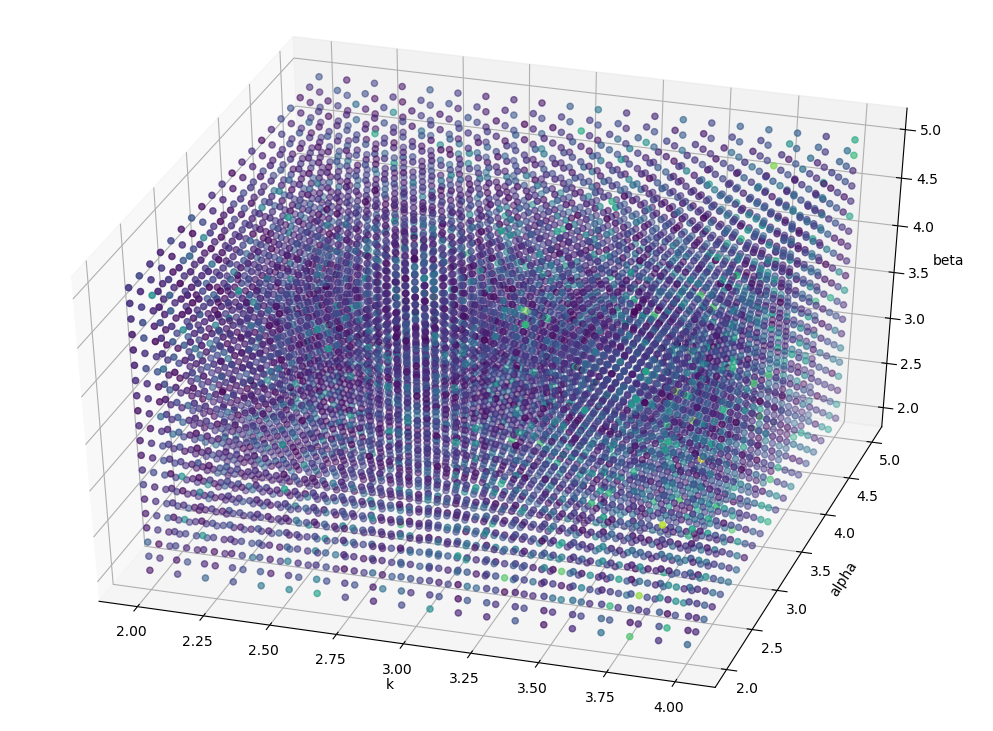
\includegraphics[width=0.8\textwidth]{./plots/ps_2N0M.png}
\caption[Parameter space search.]
{A search of a region of parameter space around $k$=3, $\alpha$=3,
$\beta$=3. The colour of each point represents a normalised scaling of
the sum of squared differences between elements of $c_0$ and $c_1$
after 5000 iterations of the simulation. The maximum value of this
metric was 0.0066; the minimum was 1.7 $\times$ 10$^{-5}$. For
comparison, the value of the metric for a guided system which
separated into two clear regions at 5000 steps was 722.}
\label{fig:ps_2N0M}
\end{figure}

I created two methods to run through the parameter space. One, called
\code{analysis/scanspace.py}, creates a json file for each parameter set, then
calls the program \code{james1c}, and finally
calls \code{sos\_centroid\_analyse()} to add each result
to \code{logs/scanspace.h5}. The problem with this method is that it
repeatedly creates the \code{morph::HexGrid}, adding lots of worthless
computation. To fix this, I wrote \code{ps\_2N0M.cpp}, which uses a
single \code{RD\_James} instance, which it re-sets after each
simulation, without having to re-compute the HexGrid. This can
evaluate 5000 timesteps of one parameter set with the Hex to Hex
spacing set to 0.02 in 1.3 seconds (on
threadbeast). \code{ps\_2N0M.cpp} runs the simulations, but it doesn't
apply the final analysis step of computing the sum of squared
differences between c0 and c1. This is carried out by
\code{analysis/ps\_2N0M\_postproc.py} and plotting by
\code{analysis/ps\_2N0M\_plot.py}. See Fig.~\ref{fig:ps_2N0M}.

%%%%%%%%%%%%%%%%%%%%%%%%%%%%%%%%%%%%%%%%%%%%%%%%%%%%%%%%%%%%%%%%%%%%%%%%%%%%%%%
\section{Two dimensional system with changed competition}

The symmetry of the terms for $\pm \alpha_i c_i$ and
$\pm \beta_i n a_i$ in
Equations \ref{eq:Karb1D_dc} \& \ref{eq:Karb1D_da} results directly
from the simple kinetic reaction:

\begin{equation} \label{eq:kinetic}
n + a_i \xrightleftharpoons[\alpha_{i}]{\beta_{i}} c_i
\end{equation}

If I want to change the competition between axons from different
thalamocortical regions, I need to consder exactly what it is about
Eq.~\ref{eq:kinetic} that I want to modify, so that the model is
changed with some sort of guiding principle.

Here are some modifications to the equations to enable competition
between regions dreamed up in just such a flagrant, un-principled way:

In the following, I'll use these definitions:

Let $\hat{a}_i$ be the sum of the branching densities of all axon
types except $i$.
%
\begin{equation}
\hat{a}_i(\mb{x},t) = \sum_{p\ne i}^N a_p(\mb{x},t)
\end{equation}
%
Define the static vector field $\mb{g}$ as:
%
\begin{equation} \label{eq:g_i}
\mb{g}_i(\mb{x}) = \sum_{j=1}^M \big(\gamma_{i,j} \nabla\rho_j(\mb{x}) \big)
\end{equation}

%%%%%%%%%%%%%%%%%%%%%%%%%%%%%%%%%%%%%%%%%%%%%%%%%%%%%%%%%%%%%%%%%%%%%%%%%%%%%%%
\subsection{Allow the branching rate of all other TC axon types to change $\dot{a}_i$}
\label{sec:comp1}

Add a term to the Karbowski equations which reduces the branching rate
change based on the proximity of branching of other TC axon types:
%
\begin{equation} \label{eq:Karb2D_dc_compo_1}
\frac{\partial c_i(\mb{x},t)}{\partial t} = -\alpha_i c_i(\mb{x},t)
+ \beta_i n(\mb{x},t)
[a_i(\mb{x},t)]^k
\end{equation}
%
\begin{equation} \label{eq:Karb2D_da_compo_1}
\frac{\partial a_i(\mb{x},t)}{\partial t}
= \nabla\vcdot\mb{J}_i(\mb{x},t) - \frac{\partial
c_i(\mb{x},t)}{\partial t} - \frac{\epsilon_i  a_i}{N-1} \sum_{p \ne i}^{N} a_p(\mb{x}, t)^l
\end{equation}
%
\begin{equation}
n(\mb{x},t) = 1 - \sum_{i=1}^{N} c_i(\mb{x}, t)
\end{equation}
%
with the flux current as given by Eq.~\ref{eq:Karb2D_J} and Neumann
boundary conditions as usual. This adds two parameter sets; $\epsilon$
and $l$. The factor $\frac{1}{N-1}$ ensures that the value of
$\epsilon$ scales with $N$.

See the binary \code{james1} for the implementation.

The additional term could result from some sort of axon-axon repulsion
as the axons grow into the cortex, or an effect that occurs only once
they are growing within the cortical layer.

An implementation of this mechanism in \code{rd\_james\_comp1.cpp}
does introduce competition quite nicely. Especially evident if $\beta$
is large.

%%%%%%%%%%%%%%%%%%%%%%%%%%%%%%%%%%%%%%%%%%%%%%%%%%%%%%%%%%%%%%%%%%%%%%%%%%%%%%%
\subsection{Add an interaction with $\nabla \hat{a}_i$}
\label{sec:comp2}

There could be an additional term to interact with the other branching
densities, to prevent the \emph{branching} overlapping (rather than
just relying on the competition between connections implied by the
definition of $n(\mb{x},t)$ in Eq.~\ref{eq:Karb2D_conserve_NM}).

Change the flux current to:
%
\begin{equation} \label{eq:Karb2D_J_NM_with_comp}
\mb{J}_i(\mb{x},t) = D \nabla a_i(\mb{x},t)
+ \frac{\bar{a}_i(\mb{x}, t) F}{N-1} \nabla \hat{a}_i(\mb{x}, t) -
a_i(\mb{x}, t) \, \mb{g}(\mb{x})
\end{equation}
%
where $\bar{a}_i$ is a sigmoid of height $h$, offset $o$ and
sharpness, $s$:
\begin{equation}
\bar{a}_i = \frac{h}{1 + e^{(o - s \, a_i)}}
\end{equation}
%
The use of the sigmoid prevents the flux current from blowing up due
to the $\nabla \hat{a}_i$ term. In this term (only), we model the idea
that there must be an upper bound on the axonal branching density.

which should be another way to add competition to the system. The idea
here is that branching density should flow away from regions where
there is a high level of branching of other TC axon types.

Note that the $\nabla \hat{a}_i$ term is positive; if branching is
high for the TC type $i$ \emph{and} for all other TC types, then
diffusion of branching away from that location should be increased.

Dropping references to space and time arguments:

\begin{equation} \label{eq:Karb2D_J_NM_with_comp_noargs}
\mb{J}_i = D \nabla a_i
+ \frac{\bar{a}_i F}{N-1} \nabla \hat{a}_i - a_i \, \mb{g}
\end{equation}

The divergence of $\mb{J}_i$ is
%
\begin{equation}
\begin{split}
\nabla\vcdot\mb{J}_i & = \nabla\vcdot \big[ D \nabla a_i + \frac{\bar{a}_i
F}{N-1} \nabla \hat{a}_i - a_i \mb{g}_i \big] \\
%
& =
D \dvrg a_i
+ \frac{F}{N-1} \nabla\vcdot \bar{a}_i \nabla \hat{a}_i
- \nabla\vcdot a_i \mb{g}_i
\end{split}
\end{equation}
%
because the divergence operator is distributive (and $D$ \& $F$ are
scalar constants).  Applying the vector calculus product rule identity to
$\nabla\vcdot\big(\bar{a}_i\nabla \hat{a}_i\big)$ and
$\nabla\vcdot\big(a_i \mb{g}_i\big)$:
%
\begin{equation}
%
\nabla\vcdot\mb{J}_i = D \dvrg a_i
%
+ \frac{F}{N-1} \big(
\bar{a}_i \dvrg \hat{a}_i + \nabla \hat{a}_i \vcdot \nabla \bar{a}_i
\big)
%
- \big(
a_i\nabla\vcdot\mb{g}_i
+
\mb{g}_i\vcdot\nabla a_i
\big)
%
\end{equation}
%
Expanding the brackets we have:
%
\begin{equation} \label{eq:divJExpanded_comp2}
\boxed{
%
\nabla\vcdot\mb{J}_i = D \dvrg a_i
%
+ \frac{F}{N-1} \bar{a}_i \dvrg \hat{a}_i
+ \frac{F}{N-1} \nabla \hat{a}_i \vcdot \nabla \bar{a}_i
%
- a_i\nabla\vcdot\mb{g}_i
- \mb{g}_i\vcdot\nabla a_i
}
\end{equation}
which gives the five terms to compute in \code{rd\_james\_comp2.h}.

Result: With the sigmoid parameters set to $h=2, o=5, s=0.5$, the
range of stable values for $F$ were $[0--6]$. At the upper end of this
range, the competition effect was very slight.

%%%%%%%%%%%%%%%%%%%%%%%%%%%%%%%%%%%%%%%%%%%%%%%%%%%%%%%%%%%%%%%%%%%%%%%%%%%%%%%
\subsection{Add an interaction with $\nabla n$}
\label{sec:comp3}

Imagine that as connections are made to the cortical dendrites, a
molecule is expressed. Axon branching should expand into areas with
low connections, so the `flux of branching' should follow the gradient
of this `connectivity molecule' from low $n$ (region with few
connection sites) to high $n$ (region with many connection sites). I've
expressed this by adding a new term to Eq.~\ref{eq:Karb2D_J_NM}:
%
\begin{equation} \label{eq:Karb2D_J_NM_with_comp3}
\mb{J}_i(\mb{x},t) = D \nabla a_i(\mb{x},t)
\boxed{-a_i(\mb{x}, t) E \nabla n(\mb{x}, t)}
 - a_i(\mb{x},t) \, \mb{g}(\mb{x})
\end{equation}
%
With the new term (boxed), it's probably worth going back to look at
the method for computing $\nabla\vcdot\mb{J}_i$. Let's drop references
to the space and time arguments ($\mb{g}_i(\mb{x})$ becomes
$\mb{g}_i$; $n(\mb{x}, t)$ becomes $n$; and so on). This allows a
tidier version of Eq.~\ref{eq:Karb2D_J_NM_with_comp3} to be written
down:
%
\begin{equation} \label{eq:Karb2D_J_NM_with_comp3_simpler}
\mb{J}_i = D \nabla a_i - a_i E \nabla n - a_i(\mb{x}, t) \mb{g}_i
\end{equation}
%
The divergence of $\mb{J}_i$ is
%%%%
\begin{equation}
\begin{split}
\nabla\vcdot\mb{J}_i & = \nabla\vcdot \big[ D \nabla a_i - a_i
E \nabla n - a_i \mb{g}_i \big] \\
%
& =
D \dvrg a_i
- E \nabla\vcdot a_i \nabla n
- \nabla\vcdot a_i \mb{g}_i
\end{split}
\end{equation}
%
because the divergence operator is distributive (and $D$ \& $E$ are
scalar constants).  Applying the vector calculus product rule identity to
$\nabla\vcdot\big(a_i\nabla n\big)$ and
$\nabla\vcdot\big(a_i \mb{g}_i\big)$:
%
\begin{equation}
%
\nabla\vcdot\mb{J}_i = D \dvrg a_i
%
- E \big(
a_i \dvrg n + \nabla n \vcdot \nabla a_i
\big)
%
- \big(
a_i\nabla\vcdot\mb{g}_i
+
\mb{g}_i\vcdot\nabla a_i
\big)
%
\end{equation}
%
Expanding the brackets we have:
%
\begin{equation} \label{eq:divJExpanded_comp3}
\boxed{
%
\nabla\vcdot\mb{J}_i = D \dvrg a_i
%
- E a_i \dvrg n
- E \nabla n \vcdot \nabla a_i
%
- a_i\nabla\vcdot\mb{g}_i
- \mb{g}_i\vcdot\nabla a_i
}
%
\end{equation}
%
which gives us 5 terms to compute in \code{compute\_divJ()} in place
of the original 3 terms in Eq.~\ref{eq:divJExpanded}.

This apprach simply increases how fast branching diffuses into free
space; the $D\nabla a_i$ term already provides diffusion of branching.

%%%%%%%%%%%%%%%%%%%%%%%%%%%%%%%%%%%%%%%%%%%%%%%%%%%%%%%%%%%%%%%%%%%%%%%%%%%%%%%
\subsection{Interaction with $\nabla{n}$ and $\hat{a}_i$ inhibits $\dot{a_i}$}
\label{sec:comp4}

Combines sections~\ref{sec:comp1} and \ref{sec:comp3}. Descending the
gradient $a_i\nabla{n}$ expands axon branching into new regions;
competition between $a_i$ and $\hat{a}_i$ should prevent excessive
branching into neighbouring regions.

%
\begin{equation} \label{eq:Karb2D_dc_comp4}
\frac{\partial c_i}{\partial t} = -\alpha_i c_i
+ \beta_i n
[a_i]^k
\end{equation}
%
\begin{equation} \label{eq:Karb2D_da_comp4}
\frac{\partial a_i}{\partial t}
= \nabla\vcdot\mb{J}_i + \alpha_i c_i - \beta_i n
[a_i]^k - \frac{\epsilon_i}{N-1} a_i \sum_{p \ne i}^{N} a_p^l
\end{equation}
%
\begin{equation} \label{eq:Karb2D_conserve_NM_comp4}
n = 1 - \sum_{i=1}^{N} c_i(\mb{x}, t)
\end{equation}
%
\begin{equation} \label{eq:divJExpanded_comp4}
%
\nabla\vcdot\mb{J}_i = D \dvrg a_i
%
- E a_i \dvrg n
- E \nabla n \vcdot \nabla a_i
%
- a_i\nabla\vcdot\mb{g}_i
- \mb{g}_i\vcdot\nabla a_i
%
\end{equation}

Note that
Eqs.~\ref{eq:Karb2D_dc_comp4}--\ref{eq:Karb2D_conserve_NM_comp4} are
not quite identical those in section~\ref{sec:comp1}. The difference
is the $\frac{1}{N-1}$ factor and the inclusion of $a_i$ in the third term of
Eq.~\ref{eq:Karb2D_da_comp4}.

This is very promising! Initial branching conditions produce reliable
regions. Initial conditions can be modified to simulate denucleated
animal; region becomes smaller, but not non-existent.

%%%%%%%%%%%%%%%%%%%%%%%%%%%%%%%%%%%%%%%%%%%%%%%%%%%%%%%%%%%%%%%%%%%%%%%%%%%%%%%
\subsection{$\hat{a}_i$ inhibits $\dot{a_i}$ \bf{more}}
\label{sec:comp5}

In the config where I'm trying to make 5 barrel rows, the competition
is less competitive than I imagine it could be. The initial condition
is a blob of each of the 5 TC types of roughly the same size and I
think the problem might be that the $\epsilon$ term is inhibiting all
5 TC types more or less equally.

This idea (to avoid attenuating the biggest $a$) didn't work but lead
me to think about bounding $a$ and the problem of a winner-takes-all
situation that is easily seen.

%%%%%%%%%%%%%%%%%%%%%%%%%%%%%%%%%%%%%%%%%%%%%%%%%%%%%%%%%%%%%%%%%%%%%%%%%%%%%%%
\subsection{Add interactions with $\nabla {a}_{{p}\ne{i}}$}
\label{sec:comp6}

A scheme similar to comp2 (section \ref{sec:comp2}). However, rather
than using the gradient $\nabla \hat{a}_i$, use all the gradients of
the other TC types, with a $\zeta$ matrix to set the strengths of
interaction.

Change the flux current to:
%
\begin{equation} \label{eq:Karb2D_J_NM_with_comp6}
\mb{J}_i(\mb{x},t) = D \nabla a_i(\mb{x},t)
+ \bar{a}_i(\mb{x}, t)  \sum_{p \ne i}  \zeta_{i,p} \nabla {a}_p(\mb{x}, t) -
a_i(\mb{x}, t) \, \mb{g}(\mb{x})
\end{equation}
%
where $\bar{a}_i$ is a sigmoid of height $h$, offset $o$ and
sharpness, $s$:
\begin{equation}
\bar{a}_i = \frac{h}{1 + e^{(o - s \, a_i)}}
\end{equation}
%
used for the same reason as in section \ref{sec:comp2}.

Dropping references to space and time arguments:

\begin{equation} \label{eq:Karb2D_J_NM_with_comp6_noargs}
\mb{J}_i = D \nabla a_i + \bar{a}_i \sum_{p \ne i} \zeta_{i,p} \nabla {a}_p - a_i \, \mb{g}
\end{equation}

The divergence of $\mb{J}_i$ is
%
\begin{equation}
\begin{split}
\nabla\vcdot\mb{J}_i & = \nabla\vcdot \big[ D \nabla a_i
+ \sum_{p \ne i} \zeta_{i,p} \bar{a}_i  \nabla {a}_p - a_i \, \mb{g} \big] \\
%
& =
D \dvrg a_i
+ \sum_{p \ne i} \zeta_{i,p} \nabla\vcdot \bar{a}_i \nabla {a}_p - \nabla\vcdot a_i \mb{g}_i
\end{split}
\end{equation}
%
because the divergence operator is distributive (and $D$ \& $\zeta$ are
scalar).  Applying the vector calculus product rule identity to
$\nabla\vcdot\big(\bar{a}_i\nabla {a}_p\big)$ and
$\nabla\vcdot\big(a_i \mb{g}_i\big)$:
%
\begin{equation}
\boxed{
%
\nabla\vcdot\mb{J}_i = D \dvrg a_i
%
+ \sum_{p \ne i} \zeta_{i,p} \big(
\bar{a}_i \dvrg {a}_p + \nabla {a}_p \vcdot \nabla \bar{a}_i
\big)
%
- \big(
a_i\nabla\vcdot\mb{g}_i
+
\mb{g}_i\vcdot\nabla a_i
\big)
%
} % boxed
\end{equation}
%
which on expansion gives $3 + 2(N-1)$ terms terms to compute
in \code{rd\_james\_comp6.h} (not yet implemented).

%%%%%%%%%%%%%%%%%%%%%%%%%%%%%%%%%%%%%%%%%%%%%%%%%%%%%%%%%%%%%%%%%%%%%%%%%%%%%%%
\subsection{$\hat{a}_i$ multiplicatively reduces diffusion of $a_i$}
\label{sec:comp7}

Change the flux current to:
%
\begin{equation} \label{eq:Karb2D_J_NM_with_comp7}
\mb{J}_i = D (1 - \sigma(\hat{a}_i)) \nabla a_i - a_i \, \mb{g}
\end{equation}

where $\sigma(\hat{a}_i)$ denotes a sigmoid function:

\begin{equation}
\sigma(a) = \frac{1}{1 + e^{(o - s \, a)}}
\end{equation}

Let $\lambda = 1 - \sigma$. Then $\nabla \vcdot \mb{J}_i$ is

\begin{equation}
\nabla\vcdot \mb{J}_i = \nabla\vcdot \big( D \lambda \nabla a_i - a_i \, \mb{g} \big)
\end{equation}

Product rules all round to give:

\begin{equation}
\boxed{
\nabla\vcdot \mb{J}_i = D\big( \lambda \dvrg a_i + \nabla
a_i \vcdot \nabla \lambda \big) - \big( a_i \nabla.\mb{g} +
\mb{g} \vcdot \nabla a_i \big)
}
\end{equation}

Ah, I added in the direct competition mechanism of
section \ref{sec:comp1} (though as refined in section \ref{sec:comp4})
too (see \code{rd\_james\_comp7.h}).

%%%%%%%%%%%%%%%%%%%%%%%%%%%%%%%%%%%%%%%%%%%%%%%%%%%%%%%%%%%%%%%%%%%%%%%%%%%%%%%
\subsection{Divisive normalization of $a_i$}
\label{sec:comp8}

Taking inspiration from the divisive normalization idea in neural
networks~\cite{carandini_normalization_2011}, where the overall
activity of a group of neurons modulates the output response of an
individual member of the group, we will use the overall branching
level of all of the axons in a layer to modulate the response, $a_i'$,
of the branching level in each element.

The response can be written out with the normalization
equation~\cite{carandini_normalization_2011}:
%
\begin{equation}\label{eq:norm}
a_i' = h \; \frac {a_i^q} {\xi^q + \textstyle \sum_j^h a_{i,j}^q }
\end{equation}
%
in which $\xi$ and $q$ are free parameters and $h$ is the number of
hex elements in the domain of computation (although $h$ could also be
chosen as a free parameter if required). Here, I'll let $\xi=0$ and $q=1$.

$a_i'$, the `branching response', then has to be used to drive
connections, in practice, it is written back into $a_i$ on every
timestep.

That gives the following set of equations to express in the code:

%
\begin{equation} \label{eq:Karb2D_dc_comp8}
\frac{\partial c_i}{\partial t} = -\alpha_i c_i
+ \beta_i n
[a_i]^k
\end{equation}
%
\begin{equation} \label{eq:Karb2D_da_comp8}
\frac{\partial a_i}{\partial t}
= \nabla\vcdot\mb{J}_i + \alpha_i c_i - \beta_i n [a_i]^k
\end{equation}
%
\begin{equation}\label{eq:norm_comp8}
a_i' = h \; \frac {a_i} {\textstyle \sum_j^h a_{i,j} }
\end{equation}
%
($a_i'$ becomes $a_i$ in the next computational step.)
%
\begin{equation} \label{eq:Karb2D_conserve_NM_comp8}
n = 1 - \sum_{i=1}^{N} c_i(\mb{x}, t)
\end{equation}
%
\begin{equation} \label{eq:divJExpanded_comp8}
%
\nabla\vcdot\mb{J}_i = D \dvrg a_i
%
- E a_i \dvrg n
- E \nabla n \vcdot \nabla a_i
%
- a_i\nabla\vcdot\mb{g}_i
- \mb{g}_i\vcdot\nabla a_i
%
\end{equation}


%%%%%%%%%%%%%%%%%%%%%%%%%%%%%%%%%%%%%%%%%%%%%%%%%%%%%%%%%%%%%%%%%%%%%%%%%%%%%%%
\subsection{Divisive normalization of $a_i$ and $\hat{a}_i$ inhibits $\dot{a}_i$}
\label{sec:comp9}

This is a combination of code in section \ref{sec:comp4} (the
competition part) and \ref{sec:comp8}.

I think I like the idea of computing $\partial c_i/\partial t$ first in the simulation,
then using that as one part of the $\partial a_i/\partial t$ computation. Also, I think
there should be an additional `branching accumulation' term to reflect
the idea that branching increases with time.

I've tried these ideas. They again suffer from the problem that
there's no upper bound on $a$ (even with the divisive
normalization).

%%%%%%%%%%%%%%%%%%%%%%%%%%%%%%%%%%%%%%%%%%%%%%%%%%%%%%%%%%%%%%%%%%%%%%%%%%%%%%%
\subsection{Upper bound on $a_i$ (with $n_a$) and $\hat{a}_i$ inhibits $\dot{a}_i$}
\label{sec:comp10}

The previous attempts at competition suggest a need for a fixed upper
limit either on the branching density per element, of of the total
branching density within a single TC type.

One option is to put a sigmoid on each $a_i$, so that it saturates at
a finite value. This could be argued to result from physical or
chemical constraints.

%%%%%%%%%%%%%%%%%%%%%%%%%%%%%%%%%%%%%%%%%%%%%%%%%%%%%%%%%%%%%%%%%%%%%%%%%%%%%%%
\subsection{Upper bound on $a_i$ (sigmoid) and $\hat{a}_i$ inhibits $\dot{a}_i$}
\label{sec:comp11}

The alternative is to let $n_c \equiv n$ and introduce a new $n_a$
such that
%
\begin{equation}
n_c = 1 - \sum_i c_i
\end{equation}
%
\begin{equation}
n_a = 1 - \sum_i a_i
\end{equation}
%
and then introduce $n_a$ into the RD equations. The quantity $n_a$ is
then the maximum density of branching permissible due to physical
and/or chemical considerations.


%%%%%%%%%%%%%%%%%%%%%%%%%%%%%%%%%%%%%%%%%%%%%%%%%%%%%%%%%%%%%%%%%%%%%%%%%%%%%%%
\section{Initial conditions}

Initial reading of the literature suggests that axons grow towards
cortex in a `guideposted manner' and then start branching once within
the cortex. This would suggest that initial conditions should be more
targeted than in the Karbowski model, with axons of type $i$ arriving
in a region expected to be region $i$, but with the possibility of
modifying the model to simulate an enucleated animal by reducing the
density of incident visual TC axons, or reducing their branching rate.

I've implemented a scheme, using 2D Gaussians of varying (symmetrical)
width, gain and location, to make masks for the initial branching
densities for the different thalamocortical axon types.

%%%%%%%%%%%%%%%%%%%%%%%%%%%%%%%%%%%%%%%%%%%%%%%%%%%%%%%%%%%%%%%%%%%%%%%%%%%%%%%
\section{Axon guidance reading}

Erzurumlu \& Gaspar~\cite{erzurumlu_development_2012} have a great
table of chronological events in the development of the whisker
barrels.

Gross topographic order is present in the projections from the
trigeminal ganglion to the whisker pad and brainstem even from E12.

Thalamocortical axons are on their way to the neocortex by E13,
passing a ``corridor'' by E13.5.

Layer IV neurons in cortex are born around E14-E15.

Thalamocortical axon pioneers arrive at prospective somatosensory
cortex around E15.

At around birth (E19 to P0), barrelette patterns emerge in principle
sensory nucleus of the trigeminal nerve.

At P1, axons of the principle sensory nucleus of the trigeminal nerve
form bands in the ventro-postero-lateral nucleus the thalamic complex
(VPM).

By P3, barreloids are visible in VPM.

Sequential ordering of pattern formation first in brainstem, then in
thalamus and finally in cortex is reviewed in Sehara \& Kawasaki, 2011.

%%%%%%%%%%%%%%%%%%%%%%%%%%%%%%%%%%%%%%%%%%%%%%%%%%%%%%%%%%%%%%%%%%%%%%%%%%%%%%%
\section{Agent based model}

It may be helpful to create a more realistic axon model, where axons
grow in a tree manner, with guidance and interactions, from physically
plausible locations in a virtual thalamus.

\section{Applying the model to whisker barrels}

Exploring how the model can speak to Whisker barrels.

Axons on their way from ventrobasal thalamus (VB) to somatosensory
cortex arrive in Layer VIb and form a `mass' of axons, with axons
branching in every direction.

I'm going to first try to model the formation of rows of axons within
this mass. It's plausible that there is an ordering within this
region, because from this region can come both the wildtype barrel
cortex \emph{or} the reversed duplicate barrel field.

\subsection{Barrel rows: $N$ 1D Gaussian waves}

This mechanism makes nice
rows. See \code{configs/whiskers/5N5M\_rows.json}. The problem is that
it requires bands of expressed guidance molecules and banded
expression isn't seen in barrel cortex by the experimentalists.

\subsection{Barrel rows: 1 guidance molecule plus competition}

With the competition described in section~\ref{sec:comp4}, it is
difficult for separate, well delineated regions to form. I'm trying to
think of an idea to make the competition between regions stronger.

One possibility is to have each TC type inhibit only selected other TC
types. This might separate the centroids of effect, leading to better
row definition.

Another idea is to introduce a chemical generated in proportion to
axon branching, which then has some finite decay time.

Or, whichever a is the highest sees no attenuation. (Implemented
as \code{rd\_james\_comp5.h}).

I think the issue is that whatever inter-TC-type attenuation there is
is swamped by the diffusion term. That branching just keeps on
spreading out...

I'll re-visit the concept of using the gradient of branching in types $j \ne i$
to influence the branching flux of type $i$ (That's in section~\ref{sec:comp2}).

\subsection{Barrel rows; 1 guidance molecule pushes right, $N$ others
push left, giving rows.}

The mechanism works quite nicely, and has the advantage of using only
graded guidance molecule expression.
See \code{configs/whiskers/5N\_boundedorder.json}
%
% BIBLIOGRAPHY
%
\selectlanguage{English}
\bibliographystyle{abbrvnotitle}
% The bibliography NoTremor.bib is the one exported from Zotero. It
% may be necessary to run my UTF-8 cleanup script, bbl_utf8_to_latex.sh
%%\bibliography{NoTremor}
%
% It produces this:
\begin{thebibliography}{1}

\bibitem{george_b._arfken_mathematical_1995}
{George B.~Arfken} and H.~J.~Weber.
\newblock {\em Mathematical {Methods} for {Physicists}}.
\newblock Academic Press, fourth edition edition, 1995.

\bibitem{karbowski_model_2004}
J.~Karbowski and G.~Ermentrout.
\newblock {\em Journal of Computational Neuroscience}, 17(3):347--363, Nov.
  2004.

\bibitem{lee_hexagonal_2014}
D.~Lee, H.~Tien, C.~Luo, et~al.
\newblock {\em International Journal of Computer Mathematics},
  91(9):1986--2009, Sept. 2014.

\bibitem{erzurumlu_development_2012}
R.~Erzurumlu and P.~Gaspar.
\newblock {\em European Journal of Neuroscience},
  35:1540--1553, Feb. 2012.

\bibitem{carandini_normalization_2011}
M.~Carandini and D.~J.~Heeger
\newblock {\em Nature Reviews Neuroscience},
  13:51--62, Nov. 2011.

\end{thebibliography}

%%% Upload the *bib file along with the *tex file and PDF on
%%% submission if the bibliography is not in the main *tex file

\end{document}
